\chapter{Implementation}
\label{ch:implementation}

This chapter explains how the simulation was designed to give users a realistic sense of what it might feel like to experience hallucinations, as reported by people living with schizophrenia. The goal was to make the experience both immersive and educational—helping users not only understand the symptoms, but also feel more empathy for those who live with them. The following sections describe how the auditory and visual elements were created, why they were chosen, and how they work together to simulate a gradual progression from subtle discomfort to more intense hallucinations.

\section{Structure of the Simulation}

The simulation was intentionally structured to create an increasingly immersive and unsettling experience that mirrors hallucinations commonly reported in schizophrenia. This design was informed by both clinical research on psychotic symptoms and educational approaches shown to foster empathy and reduce stigma among healthcare professionals.

The auditory hallucinations included in the simulation are modeled after established training tools like Patricia Deegan’s “Hearing Voices” program, which has been shown to significantly enhance empathy in both students and clinicians \cite{Hsia2022}. Building on this model, the simulation presents a series of whispered voices and confrontational phrases. These sounds are introduced gradually and increase in emotional intensity over time, reflecting research that shows emotional engagement enhances learning and empathetic understanding \cite{Skoy2016}.

In addition to auditory elements, the simulation incorporates visual hallucination features. These include colored spheres that appear unpredictably, spatial distortions using scattered dots, and a darkening of the visual field. These visual effects were inspired by clinical reports of hallucinations in schizophrenia, which often describe geometric patterns, flickering lights, and distorted or symbolic images \cite{Silverstein2021,Vanommen2019}.

The overall structure is designed to simulate both subtle and intense hallucinatory experiences. Initial symptoms—such as whispers and darkness—represent the early stages of perceptual changes. As the simulation progresses, the intensity of both auditory and visual elements increases to reflect the overwhelming nature of more severe psychotic episodes. This progression helps users understand how hallucinations can escalate over time and provides insight into the lived experience of individuals with schizophrenia.


\section{Implementation of the Simulation}
The simulation was developed in the Unity game engine, which provided the real-time rendering and interaction environment needed for an immersive experience. However, the core logic of the simulation was implemented through a set of custom C\# scripts, each responsible for specific components of the experience. The main control flow is managed by \texttt{Orchestrator.cs}, which coordinates the sequence and timing of both auditory and visual elements. Additional functionality is handled by supporting scripts: \texttt{SoundManager.cs} manages playback of hallucination voice samples; \texttt{DotManager.cs} handles the appearance and disappearance of visual noise elements; \texttt{ScreenDarkener.cs} progressively dims the field of view; \texttt{DynamicWaveDeformation.cs} introduces surface-level visual distortions; and \texttt{ObjectCollision.cs} detects user interactions with hallucinated elements.

To simulate visual anomalies like stains or darkened edges, a custom shader called

\texttt{FadeEdgeShader.shader} was created with the assistance of ChatGPT. This shader added another layer of perceptual distortion, contributing to the visual hallucination experience.

\subsection{Orchestration}
At the heart of the system lies the \texttt{Orchestrator.cs} script. This script sequences the entire simulation, controlling when sounds play, visual hallucinations appear, and environmental effects occur. The timeline was structured using IEnumerator coroutines, allowing asynchronous timed execution of events, ensuring immersive pacing without overwhelming the user too early in the experience.

\begin{lstlisting}[language=C++, caption={Orchestration Coroutine}, label={lst:orchestration}]
    IEnumerator OrchestrationSequence()
    {
        Debug.Log("Simulation started");
        yield return new WaitForSeconds(60f);
        PlayWhispers();
        // visual field is getting darker
    
        yield return new WaitForSeconds(5f);
        soundManager.PlaySound("1");
    }
    \end{lstlisting}
    

Synchronization across components ensures the user is not overwhelmed with concurrently being stimulated. For example, whispers begin before visuals, allowing users to acclimate to auditory disturbances before confronting the more visual hallucinations. Those are also paced in relation to emotional escalation in the voice samples, building tension across the timeline.
The orchestrator also manages the timing of the visual effects, ensuring that they are introduced at appropriate intervals to create a sense of progression. For example, the gradual darkening of the screen is timed to coincide with the introduction of more intense auditory hallucinations, creating a more immersive experience.
\begin{figure}[h!]
    \centering
    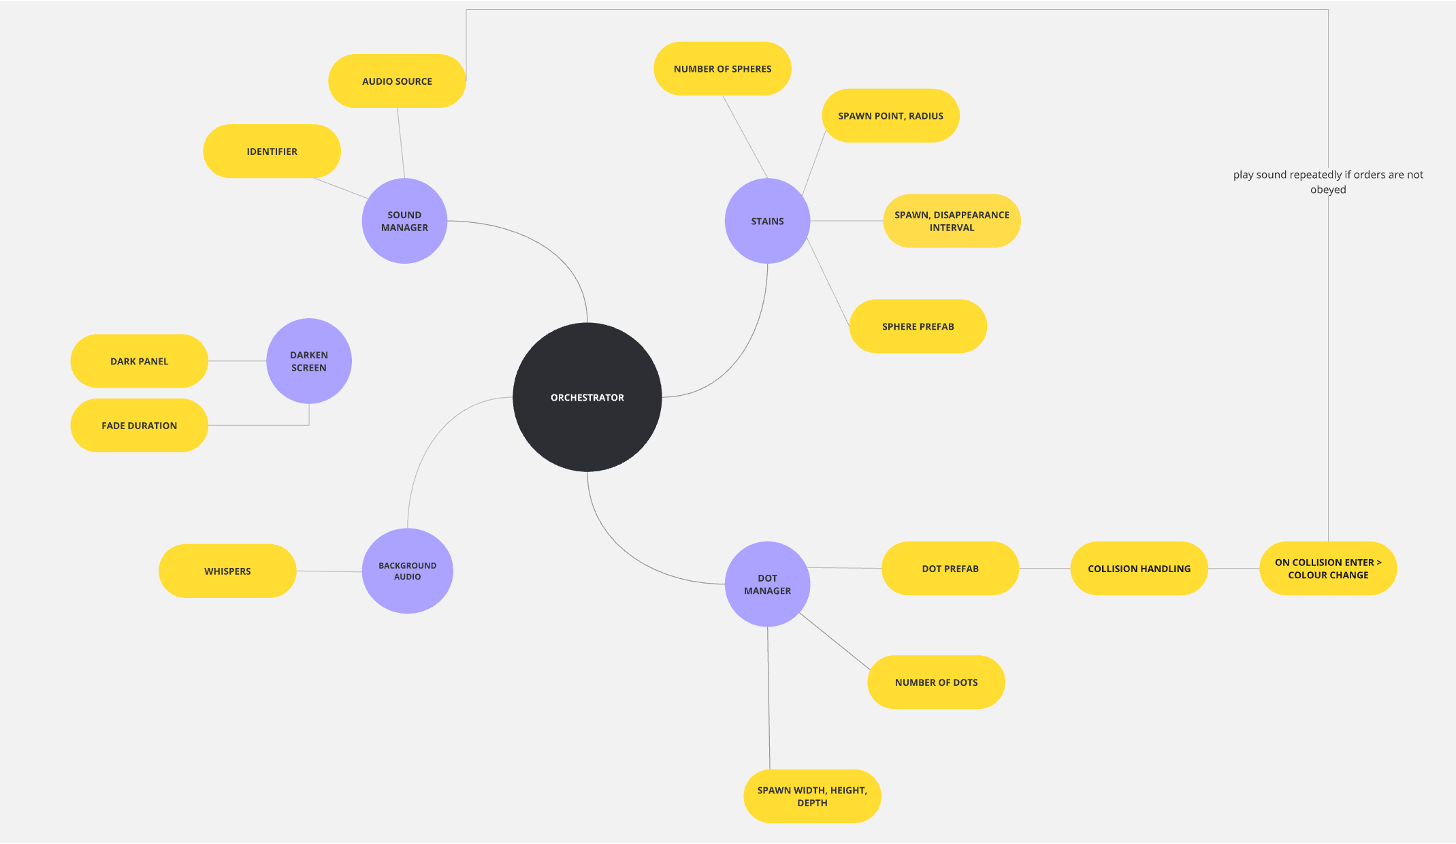
\includegraphics[width=0.8\textwidth]{../../Figures/Orch-sequence.png}
    \caption{Diagram of the Orchestrator system showing the interaction between auditory, visual, and environmental components.}
    \label{fig:orchestrator}
\end{figure}


\subsection{Auditory Hallucinations}
The auditory effects in the system are handled by the \texttt{SoundManager.cs} script. Audio files are grouped by voice type, making it easy to play back different kinds of hallucination samples. The script for these confrontational phrases was carefully drafted to include a range of emotional tones, from accusing to confused. This variety was designed to evoke a spectrum of feelings in the user, from discomfort to fear. The voices were generated using ElevenLabs, a text-to-speech AI engine \cite{elevenlabs}, which allowed for the creation of distinct emotional tones that would be difficult to achieve with traditional voice acting. Moreover, their timing is matched with visual effects to create a more immersive and realistic experience of multisensory hallucinations.

Important to mention as well is the close collaboration with the \textit{Haute école de santé Fribourg, HEdS-FR}, with whom the script was discussed with and the tone of the voices was improved upon multiple meetings and discussions we had. The team provided valuable feedback on the emotional tone and content of the voice samples, ensuring that they accurately reflected the experiences of individuals with schizophrenia.
    
\subsection{Visual Hallucinations}

The simulation includes several visual effects designed to represent different kinds of hallucinations, based on how people with schizophrenia have described their experiences. One effect, created using the \texttt{DynamicWaveDeformation.cs} script, makes the surfaces of objects appear to ripple and shift. This gives them a wavy, moving look that reflects how perception can feel distorted during hallucinations.

Another visual, controlled by \texttt{ScreenDarkener.cs}, slowly darkens the edges of the screen over time. This creates a tunnel vision effect, simulating the sense of the world closing in that some people report during intense episodes.

The \texttt{DotManager.cs} script creates random red and blue dots that float above the user. These are meant to show visual noise—unstructured, scattered visuals like the flickering lights or colored shapes that people often describe. In addition, the \texttt{Orchestrator.cs} script causes glowing spheres to appear and disappear around the user. These spheres are meant to represent sudden visual objects or presences that seem real for a short time, adding to the feeling of confusion or invasion of personal space.

All these visuals are based on research that groups hallucinations into simple effects like light flashes, geometric patterns, or more complex shapes and objects \cite{Silverstein2021,Vanommen2019}. The system is built to be flexible, so more visual effects can easily be added in future versions.

\subsection{Interaction Logic}
The interaction logic is primarily handled by the \texttt{ObjectCollision.cs} script. This script detects when the user touches one of the spheres and triggers a response. The interaction is designed to be intuitive and immediate, with the sphere changing color and stopping its sound loop upon contact.  
In addition, the script adds interactive audio that loops until the user physically interacts with an object. This mimics the frustrating and unpredictable nature of hallucinations, as often described by people experiencing psychosis.

\section{Challenges During Implementation} 
\emph{Discuss the main challenges encountered during the simulation development and how they were overcome. Highlight important coding aspects where appropriate.}

Despite careful planning, several significant challenges emerged during the development of the simulation:

\subsection{Audio Loop Management} Initially, each interactive sphere instantiated its own sound playback. This led to multiple overlapping sound loops, significantly breaking immersion and user experience. The problem arose because the audio logic was not centralized — each sphere's ObjectCollision component independently triggered audio playback upon spawning.

To solve this issue, a shared audio management system was developed, which is a static AudioSource and coroutine created within ObjectCollision.cs. This means that only one looped sound source exists, and it is globally stopped when a user interacts with any sphere.

A key logic excerpt illustrating this centralization is:

\begin{quote} \small \texttt{if (sharedAudioSource == null) { sharedAudioSource = ...; coroutineHost = this; repeatCoroutine = coroutineHost.StartCoroutine(RepeatAudio());}} \end{quote}

This ensures no duplicate sounds occur, even with multiple spheres present.

\subsection{Hand Interaction and Finger Identification} 
A second major challenge was accurately detecting when a user touched a sphere. Initially, an additional \textit{poke interaction} module was mistakenly integrated alongside Unity's built-in collision detection. This redundant system caused conflicting behavior and unpredictable touch responses. Upon deeper inspection, it was discovered that Unity’s hand collision system already assigns specific identifiers to each fingertip collider, such as \textit{HandIndex1} for the index finger. Reliable detection could therefore be implemented simply by checking the collision object's name during a collision event, rather than adding redundant interaction modules.

\begin{quote} \small \texttt{if (collision.gameObject.name.Contains("HandIndex1")) { ... }} \end{quote}

By removing unnecessary modules and using direct collision name checks, touch interactions became smooth and predictable, immediately changing the spheres color and stopping the looping sound.

\subsection{Hardware-Related Sound Privacy} During preliminary testing, the built-in speakers of the Meta Quest 3 were found to be too loud, leaking audio to the entire room and affecting non-participant observers. To address this, PhoneLook bone-conduction headphones were integrated into the simulation setup. This had the advantage that the audio is transmitted privately to the participant without occluding ambient sounds.
It also ensures immersive simulatin while respecting privacy and the testing environment.

\subsection{Spatial Placement of Sound Sources} Another significant challenge was the spatial arrangement of audio sources within the 3D simulation environment. Initially, it was difficult to orient myself correctly in Unityss Scene View, making it unclear where the sounds would originate from relative to the user's position. Proper placement was essential to create a convincing spatial auditory experience, because sounds had to feel anchored in specific locations in the environment. As the user moved, the sounds needed to remain fixed in space, enhancing realism and immersion.

To solve this, I invested time to become familiar with Unity's camera controls and 3D scene navigation.Then, the sound sources were distributed strategically across different coordinates, ensuring that different hallucinated voices would come from distinct spatial directions.

An example of the 3D placement of the sound sources in the Unity scene is shown in \autoref{fig:sound_sources}.

\begin{figure}[h!] \centering 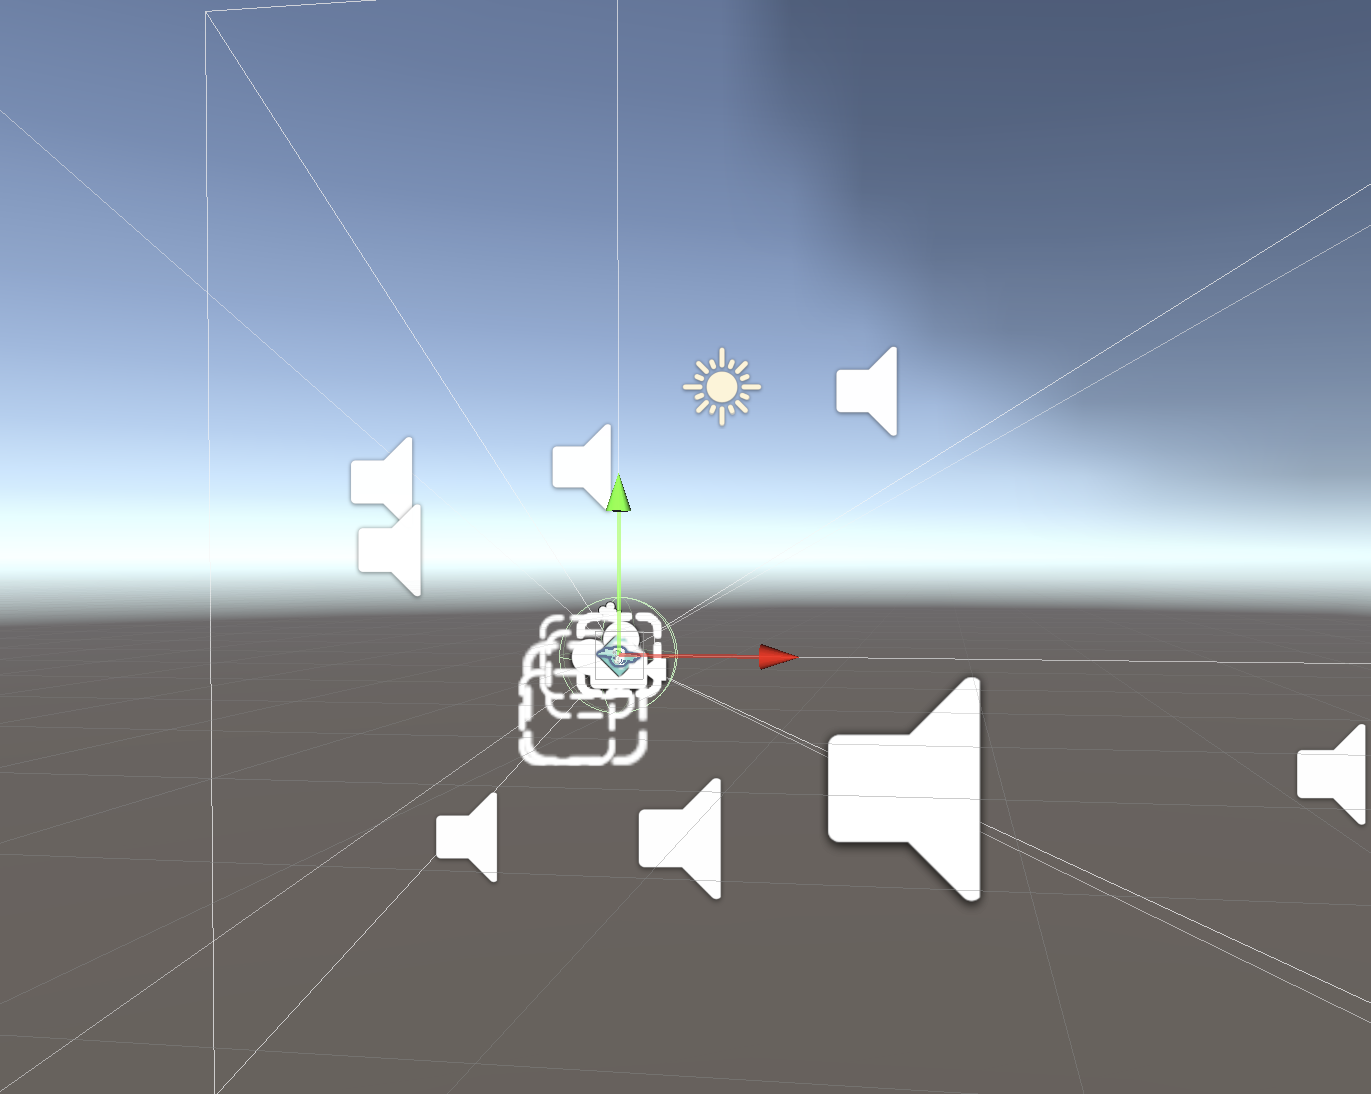
\includegraphics[width=0.8\textwidth]{../../Figures/unity-scene.png} \caption{Placement of spatial sound sources in the Unity scene for the hallucination simulation. Each speaker icon represents a sound source emitting a hallucination voice.} \label{fig:sound_sources} \end{figure}

